\documentclass[12pt]{article}


\usepackage{amsmath}
\usepackage{amssymb}
\usepackage{amsthm}
\usepackage{thmtools}
\usepackage{graphicx}
\usepackage{float}
\declaretheorem[numberwithin=section]
  {theorem, definition}
\declaretheorem{lemma, proposition, corollary}[
  style=plain,
  numberwithin=theorem
]

\title{Math 350 Ps1}
\author{Shan Gao}
\date{Fall 2023}

\begin{document}
\maketitle
\section{Problem 1}
\begin{lemma}\label{lem:1}
	If $G$ is a graph, then at least one of $G$ and $\bar{G}$ is connected.
\end{lemma}
\begin{proof}
	Let $G$ be a graph on $n$ vertices, then assume $G$ is disconnected, that means $\exists U,V \subseteq V(G)$ such that no edge in $E(G)$ can have one end in $U$ and the other in $V$. Pick any pair of vertices $u,v$ where $u \in U$ and $v \in V$, and let $w \in \bar{G}$. 
	\begin{itemize}
		\item if $w \in U$, then $(w,v) \notin E(G)$, so $(w,v) \in E(\bar{G})$
		\item if $w \in V$, then $(u,w) \notin E(G)$, so $(u,w) \in E(\bar{G})$
	\end{itemize}
	In other words, any vertex $w \in V(\bar{G})$ is adjacent to either $u$ or $v$. Furthermore, since $(uv) \notin E(G)$, then $(u,v) \in E(\bar{G})$. Thus there exists a walk between any pair of vertices $a,b \in V(\bar{G})$, if we just take 
	\begin{equation*}
		\{a , \begin{cases}
				u & (a,u) \in E(\bar{G})\\
				v & (a,v) \in E(\bar{G})
		\end{cases}, \begin{cases}
				u & (u,b) \in E(\bar{G})\\
				v & (v,b) \in E(\bar{G})
		\end{cases}, b\}
	\end{equation*}

\end{proof}
\begin{lemma} \label{lem:2}
	$G \cong H \iff \bar{G} \cong \bar{H}$
\end{lemma}
\begin{proof}
	Let $G \cong H$, then $\exists \phi \colon V(G) \to V(H)$ such that 
	\[ \forall u,v \in V(G) \text{ if }  (u,v) \in E(G) \iff (\phi(u), \phi(v)) \in E(H) \]
	then, for any $(p,q) \in E(\bar{G})$
	\begin{align*}
		(p,q) \notin E(G) &\iff (\phi(p), \phi(q)) \notin E(H)\\
				  &\iff (\phi(p), \phi(q)) \in E(\bar{H})
	\end{align*}
	Thus $\bar{G} \cong \bar{H}$,
	Conversely, $\bar{G} \cong \bar{H}$, then $\exists \phi \colon V(\bar{G}) \to V(\bar{H})$ such that
	\[ \forall u,v \in V(\bar{G}) \text{ if }  (u,v) \in E(\bar{G}) \iff (\phi(u), \phi(v)) \in E(\bar{H}) \]
	then, for any $(p,q) \in E(G)$
	\begin{align*}
		(p,q) \in E(G) &\iff (\phi(p), \phi(q)) \notin E(\bar{H})\\
				  &\iff (\phi(p), \phi(q)) \in E(H)
	\end{align*}
	thus $G \cong H$

\end{proof}
$\cong$ represents graph isomorphism
\begin{lemma}\label{lem:3}
	if $G$ is connected, then every graph in $[G]_{\cong}$ is connected. 
\end{lemma}
\begin{proof}
It's clear that any two graphs $H,F \in [G]_{\cong}$ are isomorphic. Thus there exists a bijection from $V(H) \to V(G)$ that preserves vertex adjacency, a path in $H$ is mapped to a path $F$. 
\end{proof}
Let, $F = \{ [G]_{\cong} \colon |V(G)| = n\}$ be the set of all equivalence classes of graphs on $n$ vertices.To show that there are at least $\frac{g(n)}{2}$ pairwise non-isomorphic connected graphs, essentially, by \ref{lem:3}, we want to show that there are at most $\frac{g(n)}{2}$ equivalence classes that represent a disconnected graph. If there are more than $\frac{g(n)}{2}$ pairwise non-isomorphic disconnected graphs on $n$ vertices, call them $G_1, G_2, \ldots, G_k$ where $k > \frac{g(n)}{2}$, then, by \ref{lem:2} $\bar{G_1}, \bar{G_2}, \ldots, \bar{G_k}$ are pairwise non-isomorphic connected graphs. By \ref{lem:1} and \ref{lem:2}, a disconnected graph cannot be isomorphic to it's complement, thus $\{G_1, G_2, \ldots, G_k, \bar{G_1}, \bar{G_2},\ldots, \bar{G_k}\}$ are pairwise non-isomorphic graphs, but that raises a contradiction since $|\{G_1, G_2, \ldots, G_k, \bar{G_1}, \bar{G_2},\ldots, \bar{G_k}\}| > g(n)$.  
\section{problem 2}
\begin{itemize}
	\item[(a)] False, we provide a counter example, consider the following graph $G$: 
		\begin{figure}[H]
			\centering
			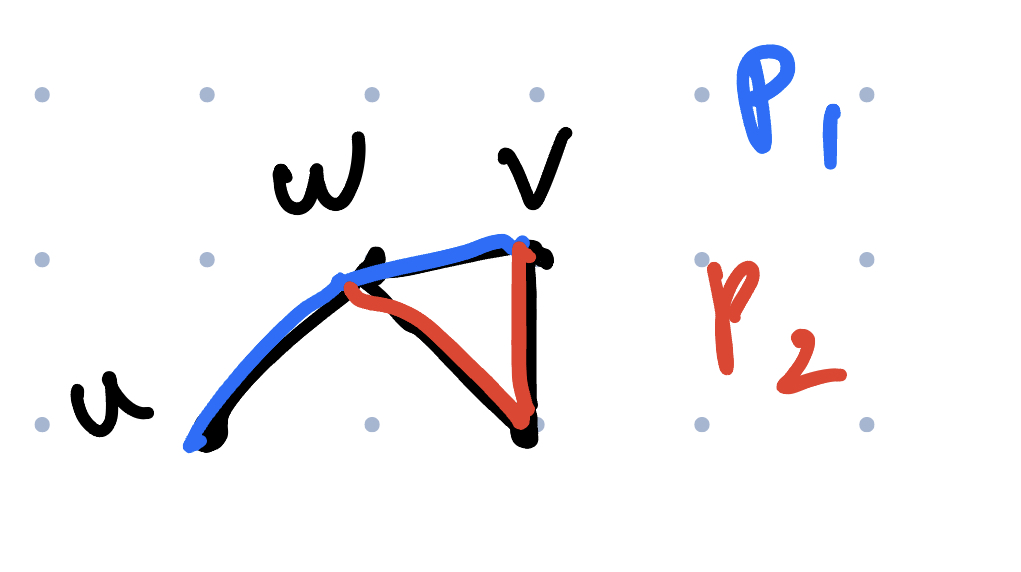
\includegraphics[width=7cm]{q2a.jpeg}
			\caption{Counterexample}
			\label{fig:q2a}
		\end{figure}
		Observe that there is an even length path $P_1$ from $u to v$ and an even length path from $v$ to $w$ but there is no even length path from $u$ to $w$. 
	\item[(b)] True, suppose towards a contradiction that there exists two disjoint paths $P_1, P_2 \subseteq G$, where $V(P_1) \cap V(P_2) = \emptyset$. Let $V(P_1) = \{u_0,u_1,u_2,\ldots,v_k\}$, and $V(P_2) = \{v_0,v_1,\ldots,v_k\}$ with vertices listed in order. There exists a path $P$ between two vertices $u_i \in V(P_1)$ and $v_j \in V(P_2)$ such that $V(P) \cap (P_1 \cup P_2) = \emptyset$, we can do this by taking $|E(P)|$ to be minimal. WLOG (since we can just invert the order of vertices) $i,j > \frac{k}{2}$, by taking the subpath $\bar{P}_1 = \{u_0,u_1,\ldots,u_j\}$ and $\bar{P}_2 = \{v_i,v_{i-1},\ldots,v_1,v_0\}$, and taking their union with $Q$, we get a new path 
		$$ \bar{P}_1 \cup Q \cup \bar{P}_2$$
		of length $i+j > k$. 
	\item[(c)] False, by counter example, observe how there exists no cycle that contains $u$ and $w$ without repeating the same vertex (the only vertex that is repeated is the start and end vertex). 
		\begin{figure}[H]
			\centering
			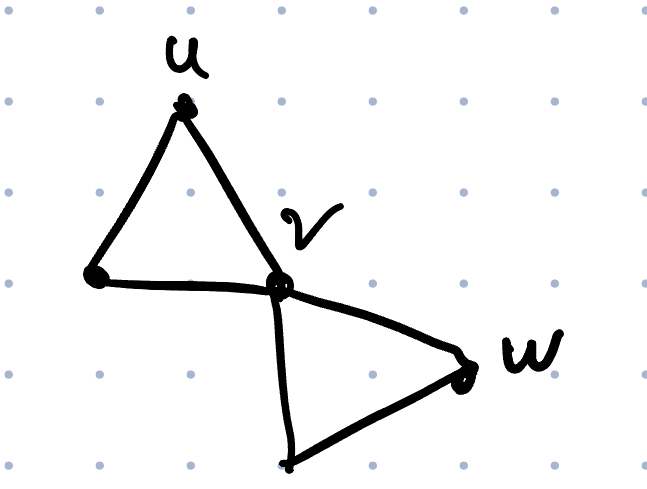
\includegraphics[width=10cm]{q2c.jpeg}
			\caption{Counterexample}
			\label{fig:2}
		\end{figure}
	\item[(d)] If the cycles don't intersect on any edge apart from $f$, then taking the union of the two cycles results in a cycle that contains $e$ and $g$. If they intersect on at least one edge other than $f$, letting $C^1$ be the cycle that contains $e,f$ and $C^2$ be the cycle that contains $f,g$. Only examining the graph $G = C^1 \cup C^2$. First of all, if we take any end vertex of $e$ and any end vertex of $g$, then there must exist two paths that \textbf{only} coincide at the start and end vertex between them. Take $u,v$ to be end vertices of $e$ and $g$ respectively, then there exists a shortest path from $u$ to a vertex $w$ where $w$ is a shared vertex between $C^1$ and $C^2$, then there must exist a path between $w$ to $v$, by connectedness. Furthermore, there must exist a shortest path from $u$ to $y$, where $y \neq w$ and $y$ is a shared vertex between the two cycles, this path is disjoint from the previous apart from $u$ (we can do this by going in the opposite direction of the cycle as compared to the path from $u$ to $w$), and then there exists a path from $y$ to $v$. It follows that there is a cycle that contains edges $e$ and $g$.
\end{itemize}
		
		\section{problem 3}
		First of all, clearly a partition of the graph into $l$ disjoint paths where $l \geq k$ exists, since you can just take the trivial partition, where every vertex is a path. Thus $l  = n$ and $n \geq k $ clearly. Let $$F = \{|\mathcal{P}| \colon \mathcal{P} \text{ is a partition of the graph $G$}, |\mathcal{P}| \geq k\}$$ be the set of possible partition sizes. By the well ordering property, there exists a minimum in this set, call it $l$. We want to show that it's equal to $k$. Suppose $l > k$, then there is a partition of $G$ into $l$ disjoint paths, $\mathcal{P}_l = \{P_1, P_2, \ldots, P_l\}$. We claim that there are at least two paths, $P_x$ and $P_y$ with adjacent endpoints, $x,y \in V(G)$. Suppose on the contrary that all the paths have pairwise non-adjacent endpoints. Then let $F = \{u_1,u_2,\ldots,u_l\}$ be the set containing an endpoint from each path, then this forms a set of $l > k$ pairwise non-adjacent vertices, which contradicts the maximality of $k$. Therefore, we can conclude there exists two paths $P_x$ and $P_y$ with adjacent endpoints, we can then take $P = P_x \cup P_y$ to form a path that contains $P_x$ and $P_y$ and is also disjoint from the other paths. Therefore, $\{P, P_3,\ldots,P_l\}$ is a valid partition of the graph into $l-1$ disjoint paths, contradicting the minimality of $l$. Therefore, we can conclude that $l = k$. 




\end{document}
